\documentclass[twocolumn,a4paper,11pt]{scrartcl}

% Language and font encoding
\usepackage[spanish,es-noshorthands]{babel}
\usepackage[utf8]{inputenc}
\usepackage[T1]{fontenc}

% Other necessary packages
\usepackage{graphicx}
\usepackage{amsmath}
\usepackage{cite}

% Additional formatting for two-column layout with centered abstract
\renewcommand{\absnamepos}{empty}  % Remove space where "Abstract" title was
\addto{\captionsspanish}{\renewcommand{\abstractname}{}} % quitar título del resumen

% Title information
\title{Relación carga-masa del Electrón}
\author{Brian David Leiva. ECFM-USAC}
\date{Abril, 2025}

\begin{document}

\twocolumn[
  \begin{@twocolumnfalse}
    \maketitle
    \begin{abstract}
    \begin{center}
    \begin{minipage}{0.6\textwidth}
En esta práctica, se estudió la deflexión de electrones en un campo magnético para determinar la relación carga-masa del electrón. Se midió la trayectoria circular de los electrones y se analizó la relación entre el campo magnético y el potencial de aceleración, manteniendo constante el radio de la órbita. Mediante estos datos, se determinó la carga específica del electrón, obteniendo un valor que permite comprender mejor las propiedades de esta partícula subatómica.
\end{minipage}
\end{center}
\end{abstract}
\end{@twocolumnfalse}
]

\section{Objetivos}

El propósito principal de esta práctica es estudiar la deflexión de electrones en un campo magnético, observando su trayectoria circular. Este análisis nos permitirá comprender mejor el comportamiento de las partículas cargadas bajo la influencia de campos magnéticos.

A partir de este estudio, nos proponemos determinar la relación entre el campo magnético B y el potencial de aceleración U de los electrones, manteniendo constante el radio r de su órbita. Esta investigación nos proporcionará información valiosa sobre la dinámica de los electrones en condiciones controladas.

Finalmente, utilizando los datos obtenidos en los objetivos anteriores, buscaremos determinar la carga específica del electrón. Este valor  nos ayudará a profundizar en nuestra comprensión de las propiedades intrínsecas de esta partícula subatómica y su comportamiento en campos electromagnéticos.

\section{Marco teórico}

El estudio de la relación carga-masa del electrón es fundamental en la física de partículas. Aunque la masa del electrón ($m_e$) es difícil de medir directamente, podemos determinar con mayor facilidad su carga específica ($\varepsilon$), definida como la relación entre su carga ($e$) y su masa:

\begin{equation}
\varepsilon = \frac{e}{m_e}
\end{equation}

Este valor nos permite calcular la masa del electrón si conocemos su carga elemental.

Cuando un electrón se mueve con una velocidad $v$ perpendicular a un campo magnético homogéneo $B$, experimenta la fuerza de Lorentz \cite{serway2018}:

\begin{equation}
F = e \cdot v \cdot B
\end{equation}

Esta fuerza, perpendicular tanto a la velocidad como al campo magnético, actúa como una fuerza centrípeta que obliga al electrón a seguir una trayectoria circular de radio $r$:

\begin{equation}
F = m_e \cdot \frac{v^2}{r}
\end{equation}

Igualando estas expresiones, obtenemos una relación entre la velocidad del electrón, su carga, masa, el radio de su órbita y el campo magnético:

\begin{equation}
\frac{e}{m_e} = \frac{v}{r \cdot B}
\end{equation}

En nuestro experimento, los electrones se aceleran en un tubo de rayos finos con potencial $U$. La energía cinética resultante es

\begin{equation}
    e \cdot U = \frac{1}{2} \cdot m_e \cdot v^2
\end{equation}

por lo que la carga específica del electrón es

\begin{equation}
\frac{e}{m_e} = 2 \frac{U}{(r \cdot B)^2}
\end{equation}

El tubo de haz fino contiene moléculas de hidrógeno a baja presión, que emiten luz al colisionar con electrones. Esto hace que la órbita de los electrones sea visible indirectamente, y su radio de órbita r puede ser medido directamente con una regla.

El campo magnético B es generado en un par de bobinas de Helmholtz y es proporcional a la corriente I en las bobinas de Helmholtz:

\begin{equation}
B = k \cdot I
\end{equation}

La dependencia del potencial de aceleración U de la corriente I, en el campo magnético del cual el radio de órbita de los electrones se mantiene a un valor constante r, se sigue tras reformular las ecuaciones (6) y (7):

\begin{equation}
    \begin{aligned}
U &= \frac{1}{2}\frac{e}{m_e} \cdot r^2 \cdot k^2 \cdot I^2 \\
U &= \alpha I^2
    \end{aligned}
\end{equation}

El factor de proporcionalidad
\begin{equation}
k = \mu_0 \cdot \left(\frac{4}{5}\right)^2 \frac{n}{R}
\end{equation}
donde $\mu_0 = 4\pi \cdot 10^{-7}$ (constante del campo magnético),
puede ser calculado ya sea desde el radio de la bobina R = 150 mm y el factor de enrollamiento n = 130 por bobina, o ser determinado registrando una curva de calibración $B = f(I)$. Esta ecuación nos permite determinar experimentalmente la relación carga-masa del electrón mediante la medición del potencial de aceleración, el radio de la órbita y el campo magnético aplicado.

La figura \ref{fig:electron_deflection} ilustra cómo la fuerza de Lorentz desvía los electrones en un campo magnético, forzándolos a seguir una trayectoria circular de radio $r$.

\section{Diseño experimental}




\subsection*{Calibración del campo magnético}
Inicialmente, se desconectan todas las unidades de suministro de energía, asegurando así la seguridad del equipo y la precisión de las mediciones. A continuación, se procede a retirar el dispositivo de medición y la bobina de Helmholtz ubicada en la parte frontal del montaje. Esto implica aflojar la conexión al tubo de haz fino y los pernos de fijación de los dos soportes. Se debe tener especial cuidado al retirar el tubo de haz fino, acomodándolo posteriormente en su estuche original para evitar daños. Una vez removidas estas piezas, se vuelve a armar la bobina de Helmholtz en la parte frontal y se restablece la conexión. 
Luego, se conecta la sonda axial B al Teslametro (con un rango de medición de 20 mT) y se procede a calibrar el punto cero del instrumento. Posteriormente, se posiciona la sonda axial B de manera paralela al campo magnético generado por las bobinas de Helmholtz, situándola en el centro del par de bobinas. 

\begin{figure}
    \centering
    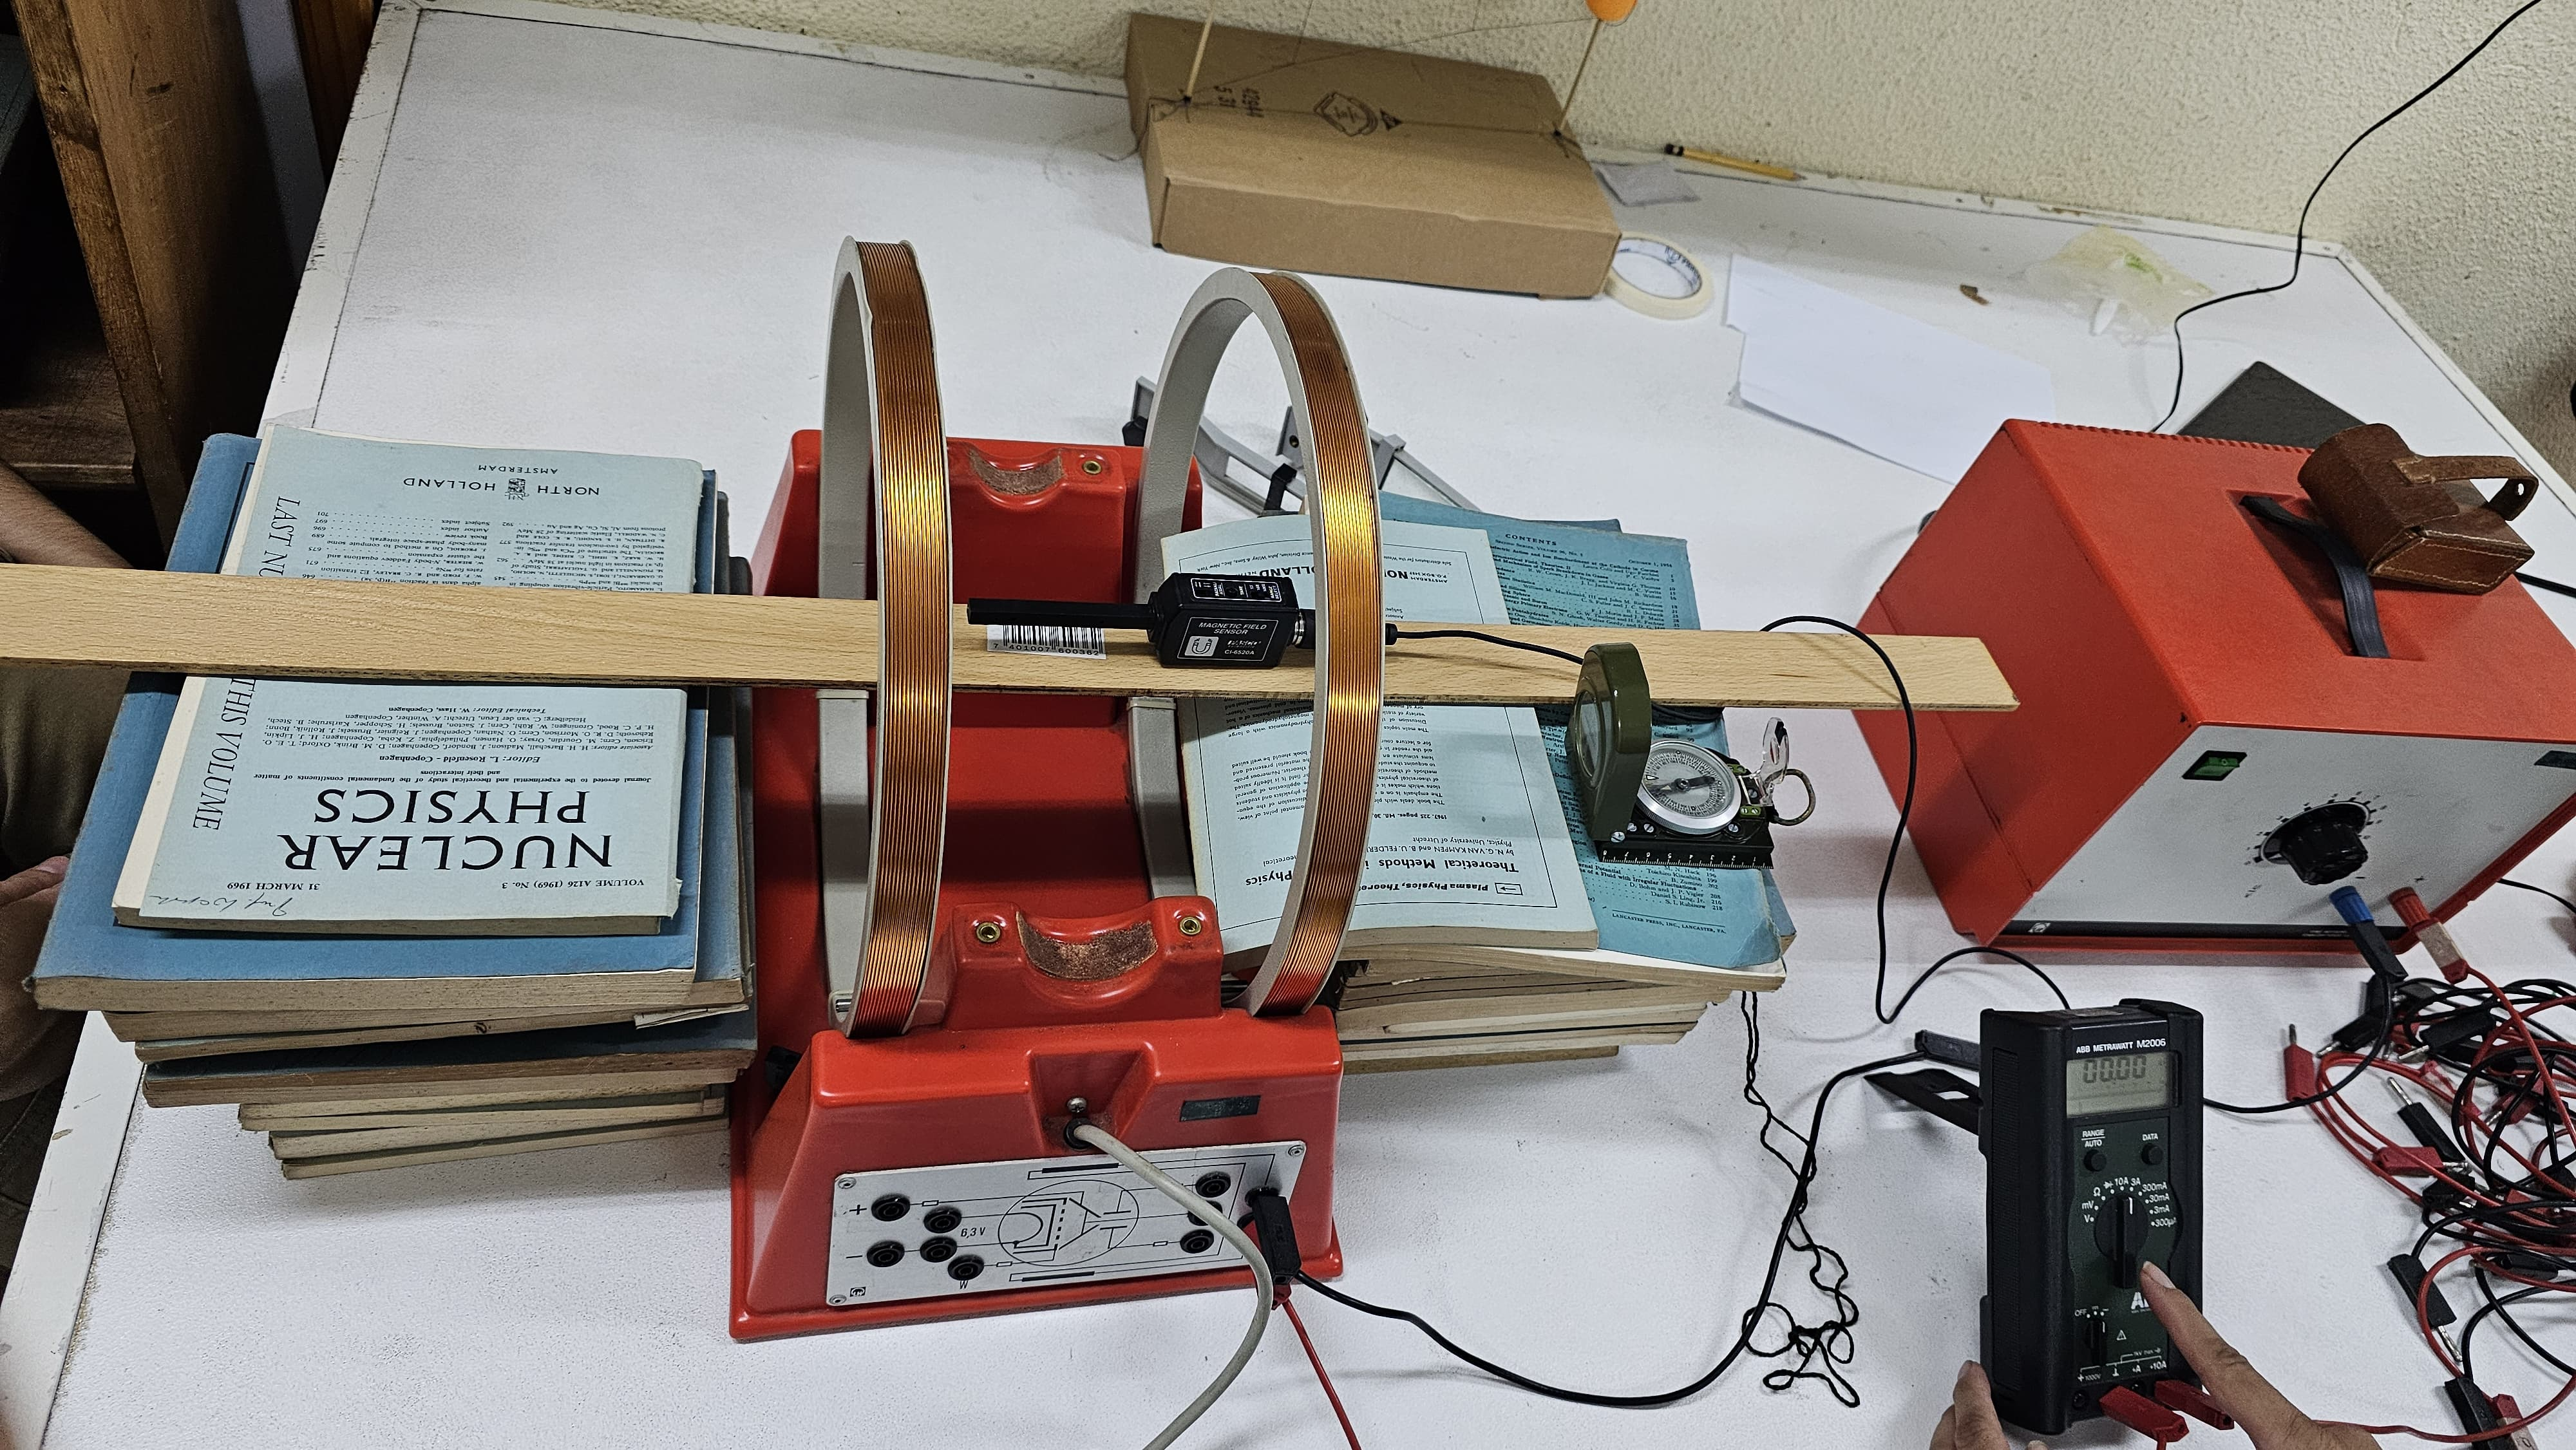
\includegraphics[width=0.4\textwidth]{montaje_exp_campo_magnetico.jpg}
    \caption{Esquema del montaje experimental para la calibración del campo magnético de Helmholtz.}
    \label{fig:electron_deflection}
\end{figure}

La figura 1 nos muestra el montaje donde tenemos las dos bobinas de Helmholtz y el sensor de campo magnético aproximadamente en el centro de la distancia entre las bobinas.

Finalmente, se incrementa la corriente en las bobinas desde 0 hasta 3 amperios en incrementos de 0.5 amperios, midiendo el campo magnético resultante en cada paso y registrando los valores obtenidos. Esto permite establecer la relación entre la corriente y el campo magnético.


\subsection*{Determinando la relación de carga-masa del electrón}

El componente central de nuesto montaje serán el tube de haz fino y las bobinas de Helmholtz.

Para alimentar y controlar nuestro sistema, utilizamos varias fuentes de poder. Una fuente de alimentación de tubo proporciona el potencial de aceleración para los electrones, mientras que una fuente de corriente continua suministra la corriente necesaria para las bobinas de Helmholtz. Además, empleamos multímetros para medir con precisión los voltajes y corrientes en diferentes puntos del circuito.

El montaje experimental se realiza en una cámara oscura para mejorar la visibilidad del haz de electrones. Es importante tener en cuenta que las bobinas de Helmholtz no deben ser sometidas a corrientes superiores a 2 A durante períodos prolongados para evitar sobrecalentamiento.

La configuración eléctrica del experimento requiere una cuidadosa conexión de los componentes. El tubo de haz fino se conecta a la fuente de alimentación de tubo, asegurando que el cátodo, el ánodo y el cilindro de Wehnelt reciban los voltajes adecuados. Las placas de deflexión del tubo se cortocircuitan al ánodo. Por otro lado, las bobinas de Helmholtz se conectan en serie con la fuente de corriente continua y un amperímetro para controlar y medir la corriente que genera el campo magnético.

Una vez realizado el montaje, el procedimiento experimental comienza con el calentamiento del tubo, que toma unos minutos. Ajustamos el voltaje en el cilindro de Wehnelt para obtener un haz de electrones bien definido y enfocado. Luego, variamos la corriente en las bobinas de Helmholtz hasta que el haz de electrones se deflecte en una órbita cerrada.

Es posible que necesitemos realizar algunos ajustes finos. Si el haz se desvía hacia el lado incorrecto, podemos invertir la polaridad del campo magnético cambiando las conexiones en la fuente de corriente continua. Si los electrones siguen una trayectoria helicoidal en lugar de circular, podemos rotar cuidadosamente el tubo de haz fino alrededor de su eje longitudinal hasta lograr una órbita circular cerrada.

Este diseño experimental nos permite controlar con precisión los parámetros relevantes para nuestro estudio: el potencial de aceleración de los electrones y la intensidad del campo magnético. Mediante la medición del radio de la órbita de los electrones bajo diferentes condiciones, podremos determinar la relación carga-masa del electrón, cumpliendo así con los objetivos de nuestra investigación.

\begin{figure}[h]
    \centering
    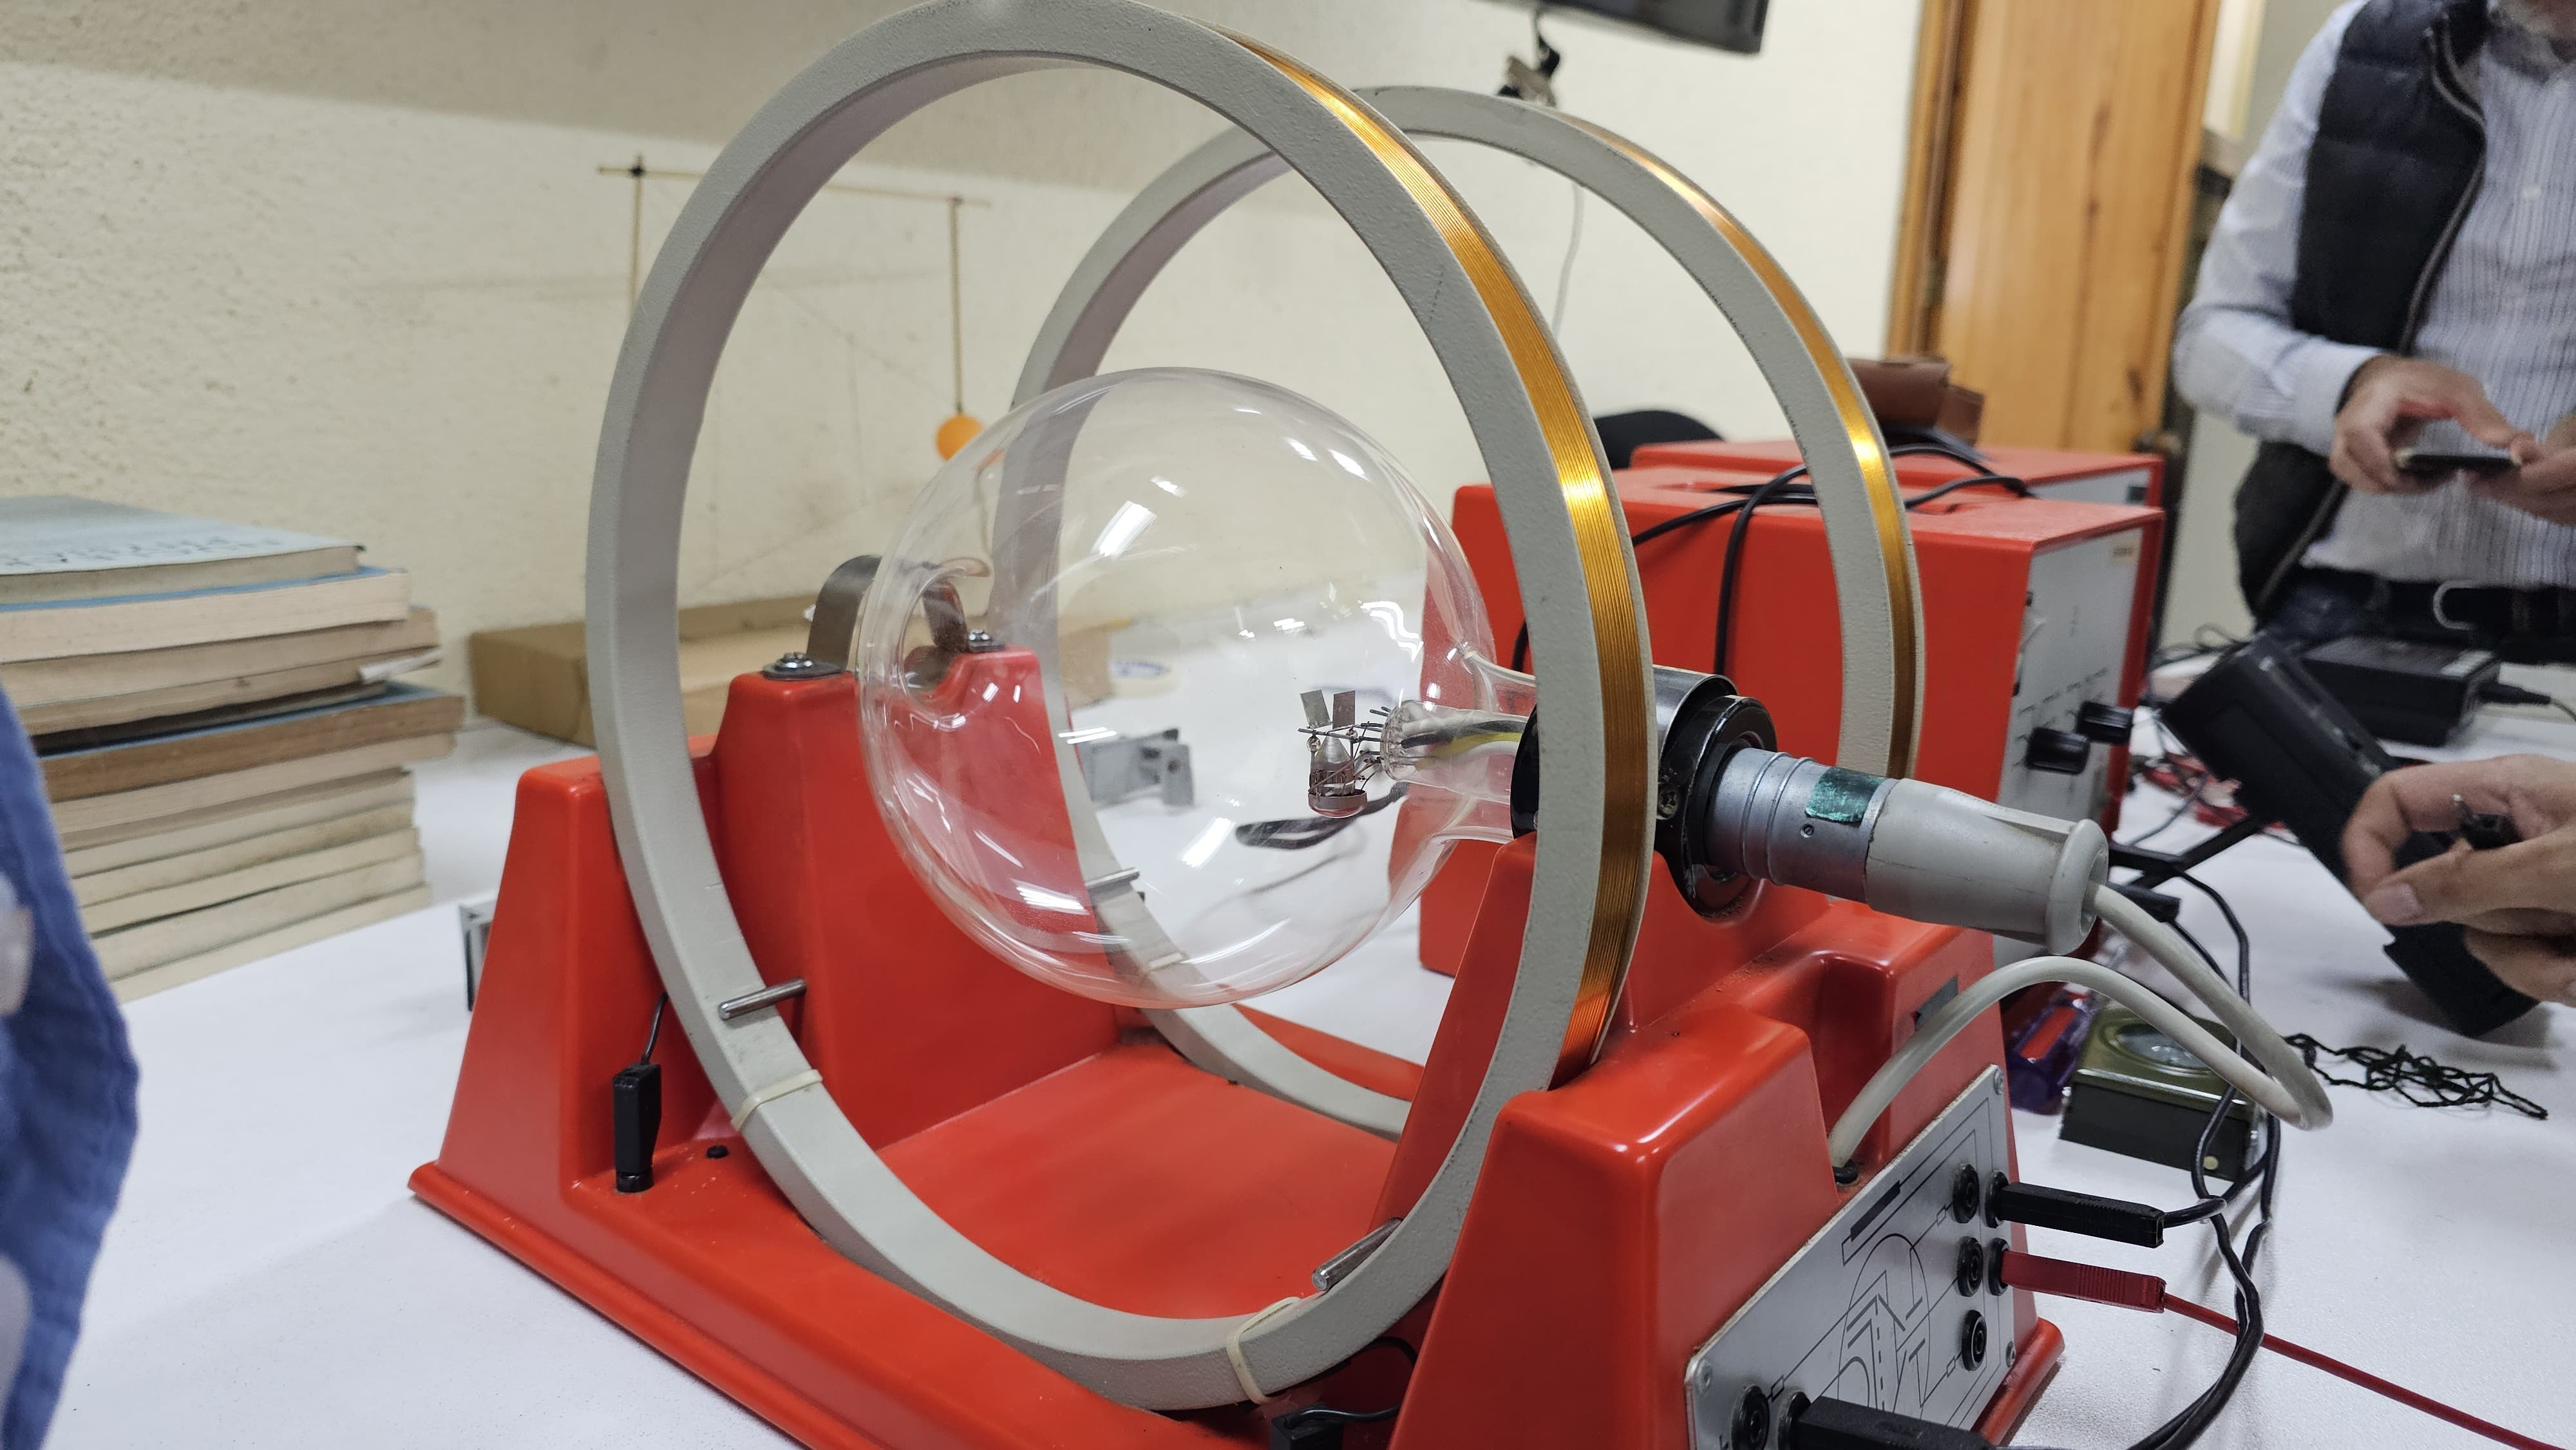
\includegraphics[width=0.8\linewidth]{montaje_exp_bobinas_helz.jpg}
    \caption{Montaje experimental para la determinación de la relación carga-masa del electrón. Se muestra el tubo de haz fino, y las bobinas de Helmholtz}
    \label{fig:experimental_setup}
\end{figure}

\subsection*{Procedimiento}

Una vez que hemos establecido nuestro montaje experimental, procedemos a realizar las mediciones siguiendo un protocolo cuidadosamente diseñado. Comenzamos ajustando el dispositivo de medición, que es crucial para determinar con precisión el diámetro de la órbita de los electrones. Movemos la corredera izquierda del dispositivo de medición de manera que su borde interior, su imagen reflejada y la apertura de escape del haz de electrones se alineen en una sola línea de visión. Este paso es fundamental para establecer un punto de referencia preciso para nuestras mediciones.

A continuación, ajustamos la corredera derecha para que la distancia entre los bordes interiores de ambas correderas sea exactamente de 6.1 cm. Esta distancia predeterminada nos servirá como referencia constante para el diámetro de la órbita de los electrones a lo largo de todo el experimento. Es importante realizar este ajuste con cuidado, ya que la precisión en esta medida afectará directamente la calidad de nuestros resultados.

Con el dispositivo de medición correctamente configurado, procedemos a alinear el haz de electrones. Para ello, enfocamos nuestra atención en el borde interior de la corredera derecha y su imagen reflejada. Ajustamos cuidadosamente la corriente de las bobinas hasta que el haz de electrones corra tangencialmente a lo largo del borde de la corredera, cubriendo su imagen reflejada. Este paso requiere paciencia y precisión, ya que la alineación perfecta del haz es crucial para obtener mediciones precisas.

Una vez lograda la alineación inicial, comenzamos nuestro proceso de medición sistemática. Partiendo del potencial de aceleración de 100 V, lo aumentamos gradualmente  hasta llegar a 300 V. Para cada valor de potencial de aceleración, ajustamos la corriente de las bobinas de modo que la órbita del haz de electrones mantenga constantemente un diámetro de 6.1 cm. Este proceso nos permite observar cómo varía la corriente necesaria en las bobinas para mantener una órbita constante a medida que cambia el potencial de aceleración de los electrones.

Durante todo este proceso, registramos cuidadosamente tanto el potencial de aceleración U como la corriente de las bobinas I para cada medición.

Es importante destacar que durante todo el procedimiento, debemos mantener una observación constante del haz de electrones. Cualquier desviación de la órbita circular o cambios en la intensidad del haz deben ser notados y corregidos inmediatamente para garantizar la consistencia de nuestras mediciones.

Este procedimiento nos permite recopilar un conjunto de datos preciso y confiable, que será la base para nuestro análisis posterior y la determinación de la relación carga-masa del electrón. La atención al detalle en cada paso del proceso experimental es crucial para minimizar errores y obtener resultados que reflejen con precisión el comportamiento de los electrones en nuestro sistema.

\begin{figure}[h]
    \centering
    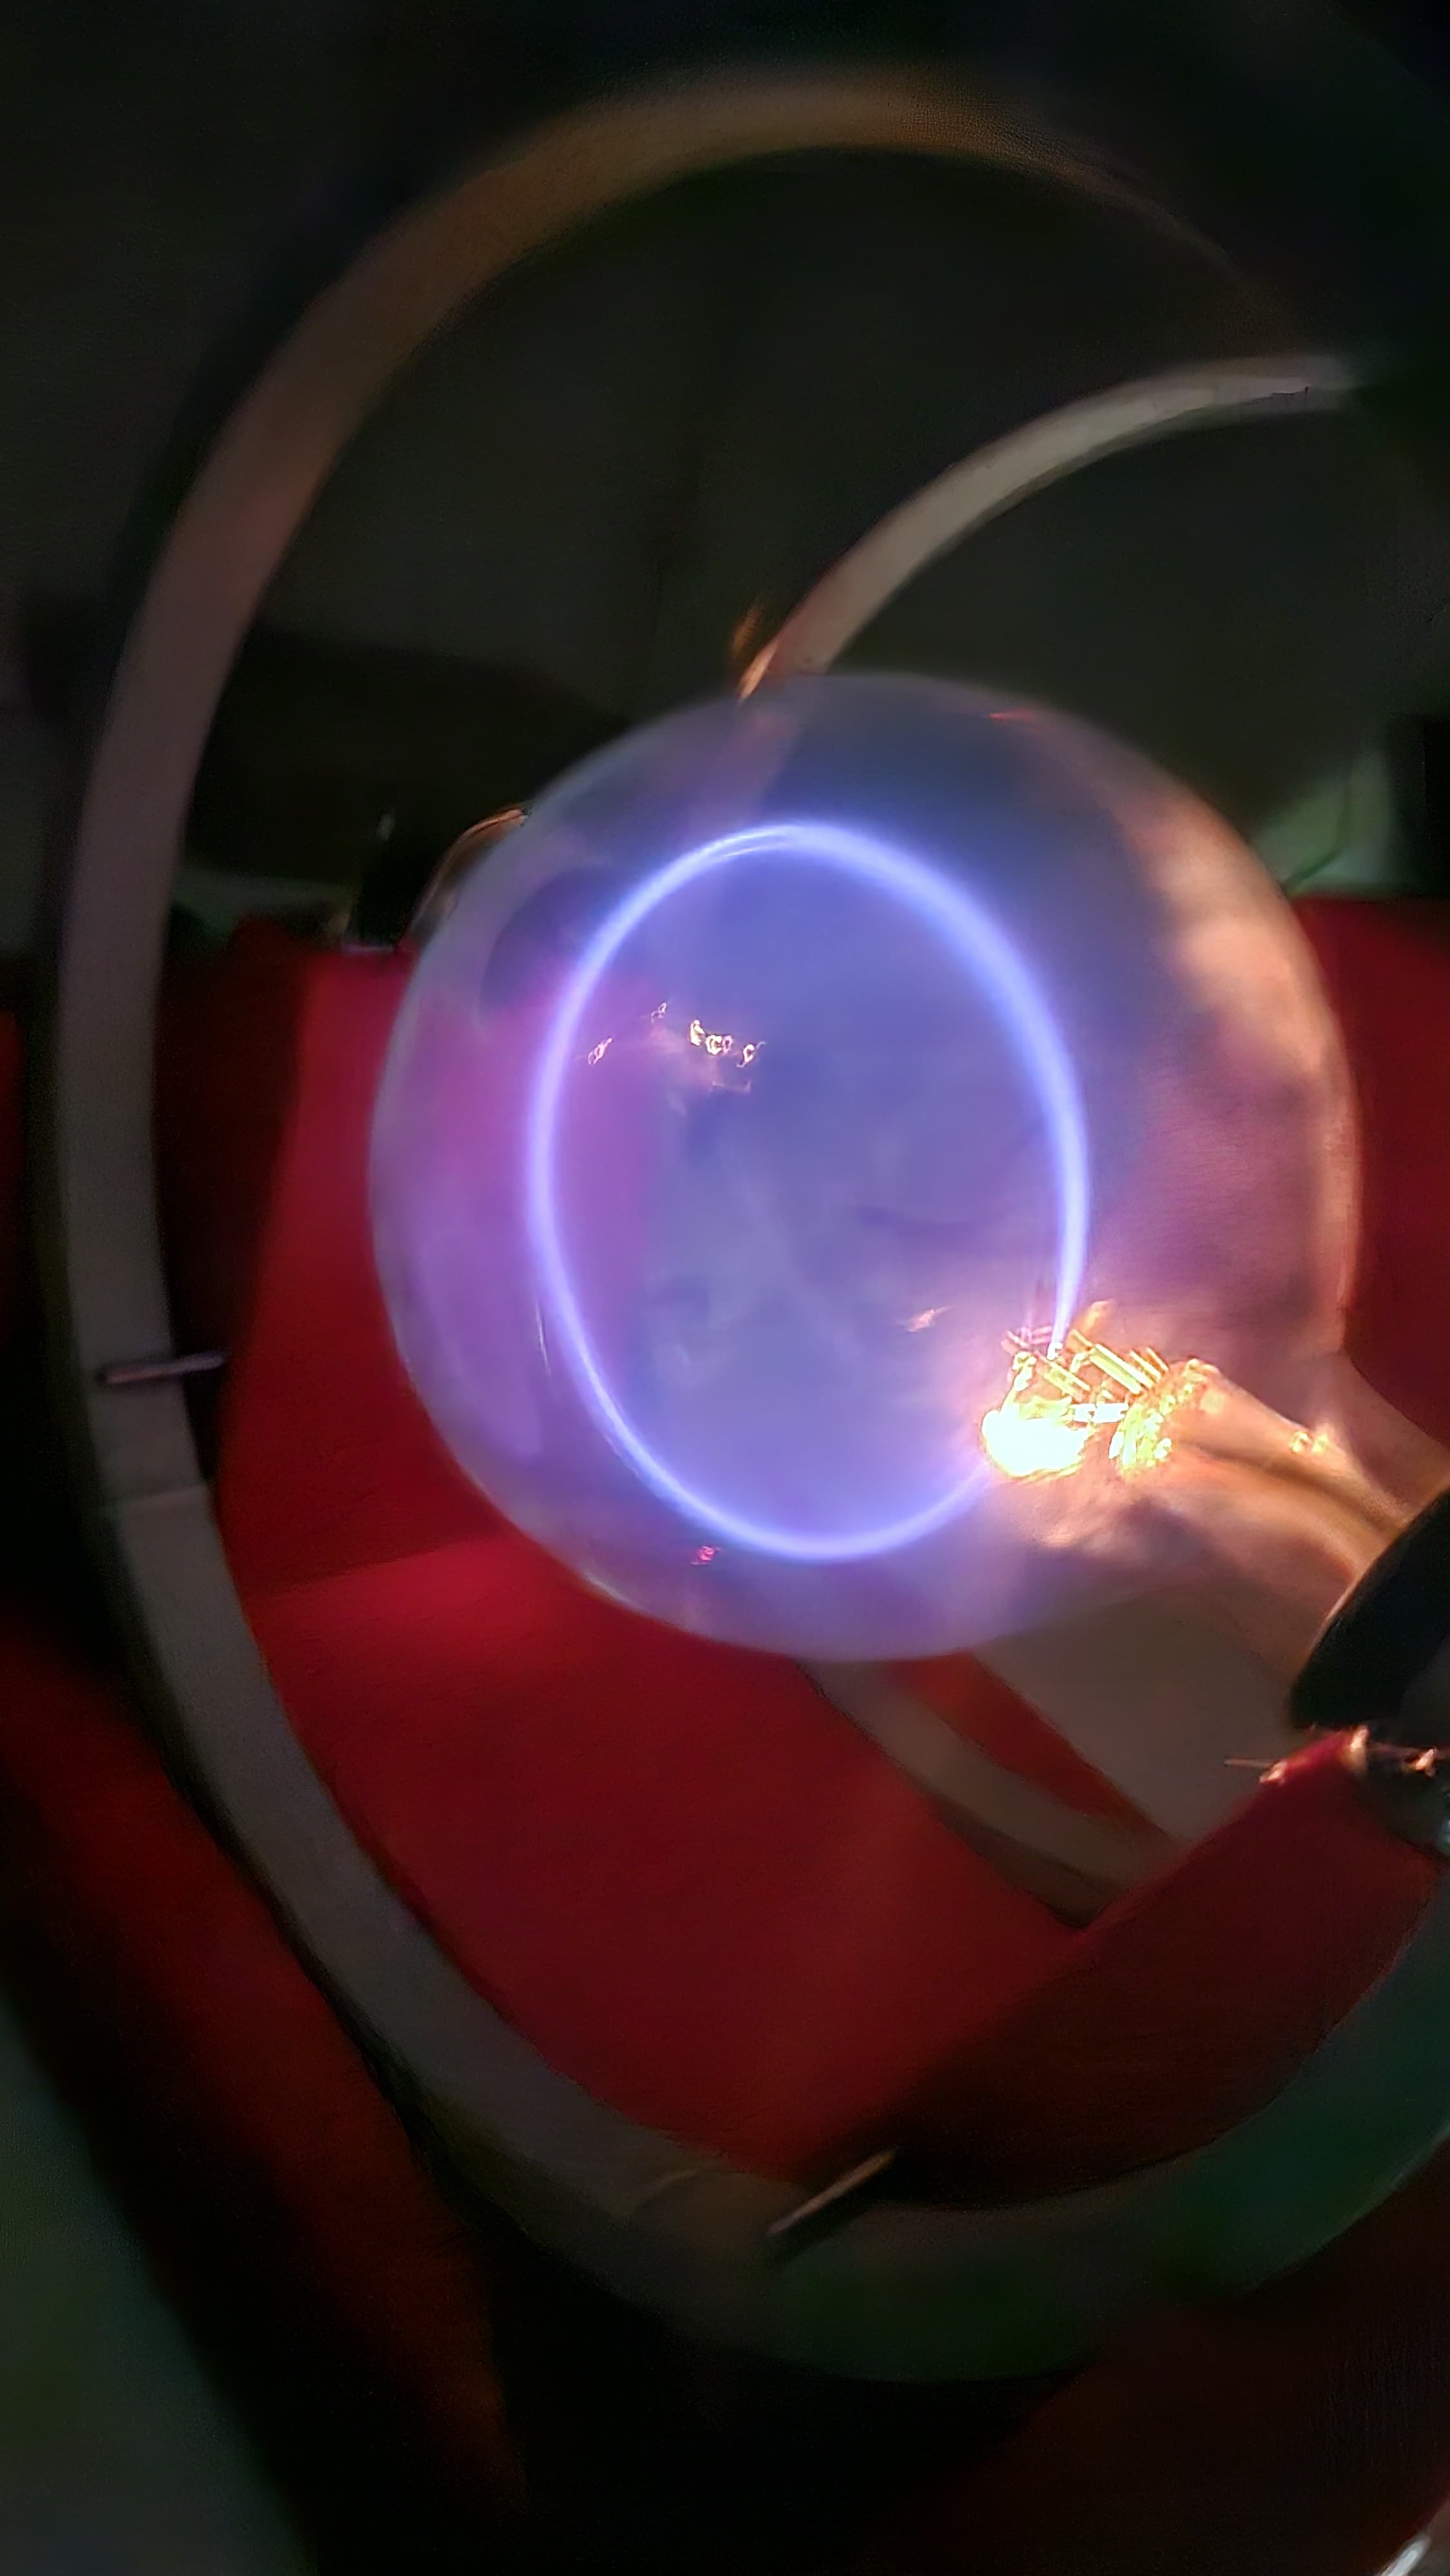
\includegraphics[width=0.8\linewidth]{haz_fino_funcionando.jpg}
    \caption{Dispositivo de medición mostrando el haz fino de electrones.}
    \label{fig:measurement_device}
\end{figure}

\section{Resultados y discusión}

Luego procedemos a analizar los datos recopilados para poder relacionar el cuadrado de la corriente con el potencial inducido. La tabla 1 muestra estos datos.

\begin{table}[h!]
\begin{tabular}{ |c| c | } 
\hline
U/V ($\pm 1$) & I/A ($\pm 0.01$) \\ 
\hline
100 & 0.74 \\ 
149 & 0.92 \\ 
180 & 1.04 \\ 
200 & 1.07 \\ 
250 & 1.19 \\ 
300 & 1.35 \\ 
\hline
\end{tabular}
\caption{Campo magnético medido (T), sobre corriente (A)}
\label{tabla:mediciones}
\end{table}



La Figura \ref{fig:U_vs_I2} muestra la relación entre el potencial de aceleración U y el cuadrado de la corriente en las bobinas I², de acuerdo con la ecuación (8) de nuestro marco teórico. Como se puede observar, los puntos experimentales se ajustan notablemente bien a una línea recta que pasa por el origen, lo cual confirma la validez de nuestro modelo teórico. El código que utilizamos para ajustar los datos se encuentra en el repositorio de GitHub asociado a este informe \cite{leiva2025}.

\begin{figure}[h]
    \centering
    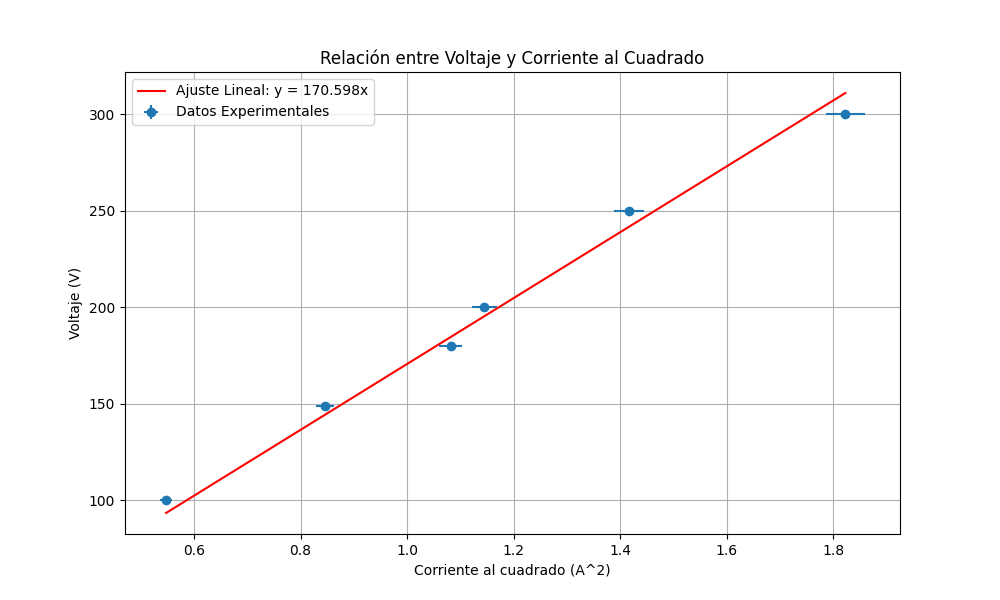
\includegraphics[width=1\linewidth]{voltaje_vs_corriente_cuadrado.png}
    \caption{Gráfico de U en función de I² mostrando la relación lineal predicha por la teoría.}
    \label{fig:U_vs_I2}
\end{figure}

El ajuste lineal de estos datos nos proporcionó una pendiente $\alpha = 170.5981$. Este valor es crucial para nuestro análisis, ya que nos permite calcular la carga específica del electrón utilizando la ecuación:

\begin{equation}
\frac{e}{m_e} = \frac{2 \cdot \alpha}{r^2 \cdot k^2}
\end{equation}

donde r es el radio de la órbita de los electrones y k es el factor de proporcionalidad entre la corriente en las bobinas y el campo magnético generado.

Para determinar el valor de k, realizamos una calibración del campo magnético de las bobinas de Helmholtz. 
La siguiente tabla muestra los resultados de la calibración del campo magnético.

\begin{table}[h!]
\centering
\begin{tabular}{ |c| c | } 
\hline
I/A $\pm0.01$ & B/mT \\ 
\hline
0.00 & -0.042 $\pm$ 0.004 \\ 
0.30 & 0.156 $\pm$ 0.002 \\ 
0.60 & 0.367 $\pm$ 0.003 \\ 
0.90 & 0.585 $\pm$ 0.002 \\ 
1.20 & 0.794 $\pm$ 0.003 \\ 
1.51 & 1.012 $\pm$ 0.003 \\ 
1.80 & 1.218 $\pm$ 0.003 \\ 
2.10 & 1.436 $\pm$ 0.003 \\ 
2.40 & 1.653 $\pm$ 0.003 \\ 
2.70 & 1.874 $\pm$ 0.002 \\ 
3.00 & 2.083 $\pm$ 0.002 \\ 
\hline
\end{tabular}
\caption{Campo magnético promedio (mT), sobre corriente (A)}
\label{tabla:AT}
\end{table}


Tras realizar un encaje lineal de los datos obtenidos y relacionarlo con la ecuación (7), obtenemos un valor de .



La Figura \ref{fig:B_vs_I} muestra los resultados de esta calibración, donde se observa una relación lineal entre el campo magnético B y la corriente I en las bobinas.

\begin{figure}[h]
    \centering
    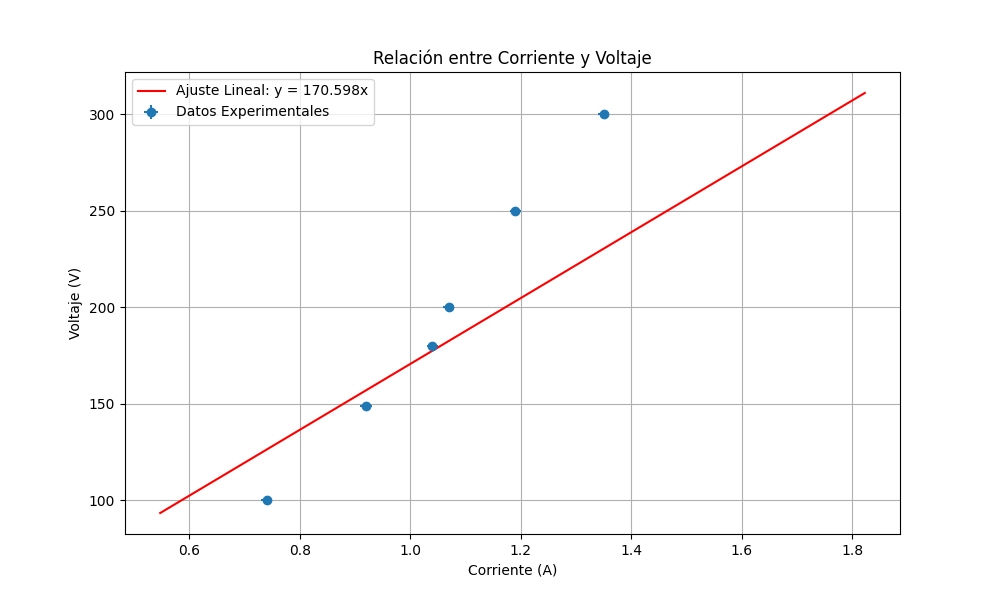
\includegraphics[width=1\linewidth]{voltaje_vs_corriente.png}
    \caption{Calibración del campo magnético: B en función de I.}
    \label{fig:B_vs_I}
\end{figure}

El ajuste lineal de estos datos de calibración nos proporcionó un valor de $k =  (7.13 \pm 0.58) E-04$ mT/A. Utilizando este valor experimental de k, junto con el radio de la órbita r = 0.061 cm y la pendiente $\alpha$ obtenida anteriormente, calculamos la carga específica del electrón:

\begin{equation}
\frac{e}{m_e} = 1.8 \pm 0.8 E11  
\end{equation}


Este valor está en el mismo orden de magnitud que el valor aceptado de la carga específica del electrón (1.76 E11 C/kg). Esto nos da confianza en la validez general de nuestro método experimental y en la robustez de nuestros resultados.

La ligera diferencia entre nuestros resultados y el valor aceptado puede deberse a varios factores. Por un lado, nuestro experimento asume que los electrones siguen una trayectoria perfectamente circular, lo cual puede no ser completamente cierto debido a pequeñas inhomogeneidades en el campo magnético. Además, la presencia de campos eléctricos residuales o la influencia del campo magnético terrestre podrían introducir pequeñas desviaciones en la trayectoria de los electrones.

A pesar de estas limitaciones, nuestro experimento ha demostrado ser una herramienta valiosa para la determinación de la carga específica del electrón. La consistencia de nuestros resultados con la teoría y con los valores aceptados valida la eficacia de nuestro enfoque experimental y subraya la importancia de este tipo de experimentos en la enseñanza y comprensión de la física de partículas cargadas.

\section{Conclusiones}
En conclusión, hemos logrado determinar la carga específica del electrón ($e/m_e$) utilizando un experimento basado en la deflexión de un haz de electrones en un campo magnético uniforme. El valor experimental obtenido, $(1.8 \pm 0.8) \times 10^{11}$ C/kg, se encuentra dentro del rango aceptado de $(1.76 \pm 0.01) \times 10^{11}$ C/kg, lo que valida el procedimiento experimental y la precisión de las mediciones realizadas.

Este experimento demostró la relación directa entre la corriente aplicada a las bobinas de Helmholtz, la intensidad del campo magnético generado, y el radio de curvatura del haz de electrones. El ajuste lineal de los datos obtenidos permitió obtener un valor experimental de la pendiente ($k$) de la relación campo magnético-corriente, confirmando la linealidad esperada.


Este experimento proporciona una valiosa herramienta pedagógica para comprender los principios fundamentales de la física de partículas cargadas y para aplicar conceptos como la fuerza de Lorentz y el movimiento circular uniforme. La consistencia de nuestros resultados con la teoría y los valores aceptados refuerza la validez de nuestro enfoque experimental y subraya la importancia de este tipo de prácticas en la enseñanza de la física.

\bibliographystyle{ieeetr}
\bibliography{referencias}  

\end{document}